\section{Quy trình làm sạch và tiền xử lý dữ liệu}

\subsection{Tổng quan quy trình}

Dữ liệu thô sau khi thu thập trải qua một pipeline tiền xử lý hai nhánh song song: nhánh văn bản và nhánh hình ảnh. Mỗi nhánh có các bước xử lý đặc thù phù hợp với đặc điểm của từng loại dữ liệu.

\subsection{Tiền xử lý dữ liệu văn bản}

\subsubsection{Loại bỏ trùng lặp và lọc dữ liệu nhiễu}

Hiện tượng đánh giá trùng lặp xuất hiện tần suất cao trên các nền tảng thương mại điện tử, chủ yếu phát sinh từ các chiến dịch tăng tương tác ảo hoặc do vòng lặp cơ học của công cụ cào dữ liệu. Để giải quyết vấn đề này, nhóm áp dụng thuật toán băm MD5 trực tiếp lên nội dung trường \texttt{text} sau khi đã chuẩn hóa cơ bản. Mỗi bản ghi được ánh xạ thành một chuỗi thập lục phân 32 ký tự duy nhất. Thuật toán tiến hành quét toàn bộ tập dữ liệu, các bản ghi có chung giá trị băm sẽ bị loại bỏ và chỉ giữ lại một đại diện duy nhất. Phương pháp này đảm bảo khả năng lọc trùng chính xác tuyệt đối với độ phức tạp thời gian $\mathcal{O}(n)$, tối ưu hóa tốc độ xử lý trên không gian dữ liệu lớn. Kết quả thực nghiệm cho thấy hệ thống đã phát hiện và loại bỏ 4611 bản ghi trùng lặp, giữ lại 4775 mẫu dữ liệu độc lập.

Tiếp nối bước lọc trùng, hệ thống tiến hành thanh lọc các mẫu dữ liệu nhiễu. Các đánh giá chỉ chứa khoảng trắng hoặc có độ dài vật lý nhỏ hơn hoặc bằng hai ký tự được xác định là thiếu hụt thông tin ngữ nghĩa. Việc giữ lại các mẫu này sẽ gây nhiễu cho không gian vector nhúng của mô hình ngôn ngữ sau này. Quá trình lọc đã loại bỏ thêm 40 bản ghi không đạt tiêu chuẩn, đưa kích thước tập dữ liệu về con số 4735 mẫu hoàn thiện.

\subsubsection{Xử lý dữ liệu khuyết thiếu và đồng bộ định dạng}

Phân tích thống kê mô tả chỉ ra sự chênh lệch lớn về tỷ lệ khuyết thiếu giữa các trường thông tin. Dữ liệu đánh giá thương mại điện tử mang đặc thù tự nguyện, người dùng thường có xu hướng chỉ để lại điểm số thay vì viết nhận xét chi tiết hoặc tải lên hình ảnh đính kèm. Dựa trên đặc tính này, nhóm đề xuất các chiến lược xử lý cụ thể cho từng trường dữ liệu như được trình bày chi tiết trong Bảng 3.2.

\begin{center}
\renewcommand{\arraystretch}{1.4}
\begin{tabularx}{\textwidth}{|l|c|X|}
\hline
\rowcolor[HTML]{E8E8E8}
\textbf{Trường dữ liệu} & \textbf{Tỉ lệ thiếu} & \textbf{Chiến lược xử lý} \\
\hline
\texttt{text} & $\sim$34.02\% & Xóa toàn bộ bản ghi do không thể suy diễn đặc trưng ngữ nghĩa cho mô hình học sâu \\
\hline
\texttt{image\_urls} & $\sim$58.28\% & Giữ nguyên cấu trúc rỗng vì hành vi đánh giá không đính kèm hình ảnh là hoàn toàn hợp lệ \\
\hline
\texttt{date} & $\sim$0.51\% & Chuyển đổi về định dạng thời gian chuẩn và loại bỏ các giá trị lỗi không thể ép kiểu \\
\hline
\texttt{rating} & 0.00\% & Ép kiểu dữ liệu về số nguyên và giới hạn nghiêm ngặt miền giá trị hợp lệ từ 1 đến 5 \\
\hline
\end{tabularx}
\captionof{table}{\centering Tỉ lệ dữ liệu khuyết thiếu và chiến lược xử lý tương ứng}
\end{center}

Quy trình đồng bộ hóa kiểu dữ liệu và định dạng vật lý là bước tiếp theo nhằm đảm bảo các thao tác tính toán ma trận trong quá trình huấn luyện không bị gián đoạn bởi các ngoại lệ lập trình. Các thao tác chuyển đổi kiểu dữ liệu được thực hiện chi tiết như sau:

\begin{itemize}[labelsep=10pt, leftmargin=2cm]
    \item Cột \texttt{date}: chuyển sang kiểu thời gian \texttt{datetime64} thông qua hàm ép kiểu với tham số bỏ qua lỗi. Tổng cộng 134 bản ghi có giá trị thời gian không hợp lệ được điền bổ sung bằng giá trị liền kề trước đó.
    \item Cột \texttt{rating}: chuyển sang kiểu số nguyên, điền giá trị 0 cho các ô trống, sau đó thiết lập bộ lọc chỉ giữ lại các bản ghi có điểm đánh giá trong khoảng từ 1 đến 5. Có 17 bản ghi bị loại bỏ do mang giá trị nằm ngoài khoảng hợp lệ.
    \item Cột \texttt{text}: thực hiện cắt bỏ khoảng trắng ở hai đầu chuỗi và loại bỏ 211 bản ghi có nội dung rỗng sau khi hoàn tất các bước làm sạch cơ bản.
\end{itemize}

\subsubsection{Chuẩn hóa và làm sạch văn bản}

Quá trình chuẩn hóa văn bản tiếng Việt từ nguồn đánh giá thương mại điện tử được thực thi qua module \texttt{TextCleaner}. Để đảm bảo hiệu năng xử lý trên tập dữ liệu quy mô lớn, hệ thống áp dụng kỹ thuật lập trình song song đa luồng thông qua thư viện \texttt{pandarallel}. Quy trình làm sạch bao gồm các bước cốt lõi sau:

\begin{enumerate}[labelsep=10pt, leftmargin=2cm]
    \item Ép kiểu dữ liệu về chuỗi an toàn và xử lý các giá trị rỗng.
    \item Chuyển đổi toàn bộ văn bản về định dạng chữ thường.
    \item Lọc bỏ các liên kết trang web, thẻ định dạng ngôn ngữ đánh dấu siêu văn bản, số điện thoại, thư điện tử và các ký tự điều khiển ẩn.
    \item Ánh xạ biểu tượng cảm xúc theo ngữ cảnh thương mại điện tử. Các biểu tượng phổ biến được chuyển đổi trực tiếp sang các từ khóa tiếng Việt mang ngữ nghĩa tương đương. Các biểu tượng không nằm trong từ điển định nghĩa trước sẽ bị xóa hoàn toàn nhằm ngăn chặn tình trạng phình to không gian nhúng.
    \item Bảo toàn nguyên trạng các từ vựng đặc thù của miền thương mại điện tử như \texttt{shop}, \texttt{ok}, \texttt{okie}, \texttt{sp}, \texttt{ship}, \texttt{shipper}. Việc không áp đặt luật chuẩn hóa cứng lên nhóm từ này giúp mô hình ngôn ngữ nắm bắt chính xác ngữ cảnh giao tiếp thực tế.
    \item Rút gọn các chuỗi ký tự bị lặp lại quá dài thành dạng chuẩn mực.
    \item Loại bỏ các ký tự đặc biệt, chỉ giữ lại bảng chữ cái tiếng Việt, chữ số và các dấu câu cơ bản.
    \item Xóa bỏ các khoảng trắng dư thừa trong câu.
\end{enumerate}

Điểm cải tiến nổi bật của quy trình này nằm ở chiến lược xử lý biểu tượng cảm xúc. Thay vì sử dụng các thư viện dịch biểu tượng tự động sinh ra các chuỗi ký tự tiếng Anh dài gây phân mảnh không gian từ vựng, hệ thống ánh xạ trực tiếp sang token tiếng Việt. Phương pháp này giúp bảo toàn tín hiệu cảm xúc và tương thích tối đa với không gian từ vựng của các mô hình Transformer ở giai đoạn sau.

\subsubsection{Đánh giá tác động chuẩn hóa}

Việc định lượng tác động của bước chuẩn hóa là yêu cầu thiết yếu nhằm xác thực tính hợp lý và hiệu quả của toàn bộ quy trình. Hệ thống tiến hành đo lường độ nén từ vựng thông qua tỷ lệ suy giảm số lượng đơn vị từ độc lập.

Kết quả thực nghiệm cho thấy, kích thước không gian từ vựng ban đầu từ 6448 đơn vị đã giảm xuống còn 4804 đơn vị sau khi chuẩn hóa, tương đương mức độ tinh gọn đạt 25,50 phần trăm. Sự suy giảm này minh chứng cho việc các biến thể từ vựng do lỗi gõ hoặc từ lóng đã được hợp nhất thành công về dạng chuẩn mực.

\begin{figure}[htbp]
    \centering
    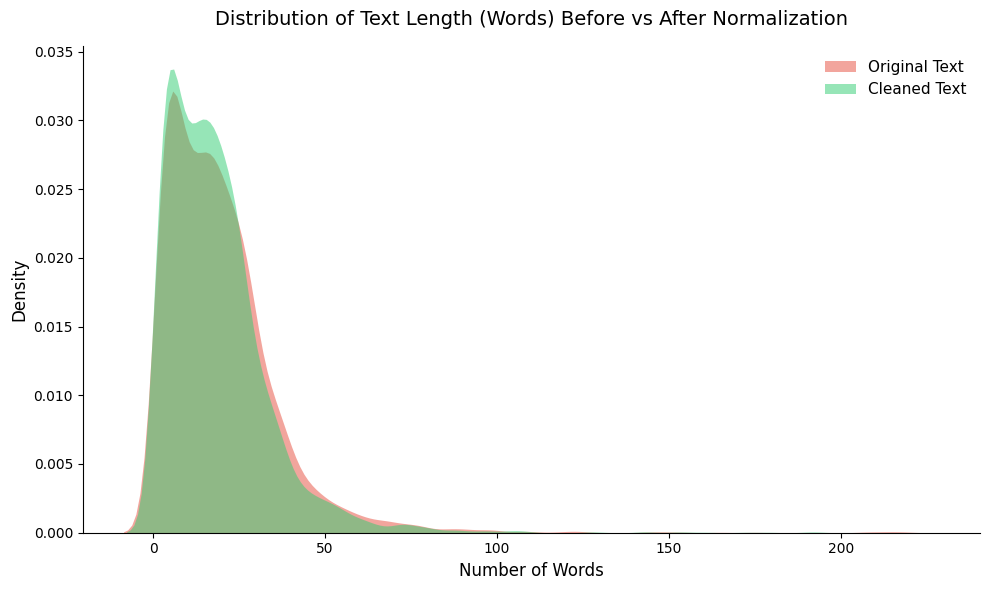
\includegraphics[width=0.85\textwidth]{graphics/kde_normalization_impact.png}
    \caption{Phân phối độ dài văn bản trước và sau khi chuẩn hóa}
    \label{fig:kde_normalization_impact}
\end{figure}

Bên cạnh đó, phân tích sự dịch chuyển phân phối độ dài văn bản qua biểu đồ mật độ hạt nhân cho thấy đường phân phối sau chuẩn hóa có xu hướng dịch nhẹ và hội tụ hơn. Điều này xác nhận rằng các kỹ thuật loại bỏ nhiễu vật lý đã làm giảm độ dài tổng thể của văn bản nhưng vẫn duy trì được sự đồng đều, không gây tổn thất các thành tố ngữ nghĩa nền tảng của đánh giá.

\subsubsection{Đánh giá và định hướng chiến lược phân mảnh văn bản}

Tiếng Việt là một ngôn ngữ đơn lập, trong đó ranh giới giữa các âm tiết được phân tách bằng khoảng trắng. Tuy nhiên, một đơn vị từ mang ngữ nghĩa hoàn chỉnh có thể bao gồm nhiều âm tiết ghép lại. Việc phụ thuộc vào kỹ thuật phân mảnh theo khoảng trắng tiêu chuẩn của tiếng Anh là thiếu tối ưu đối với đặc thù ngôn ngữ này. Nhóm tiến hành đánh giá thực nghiệm ba chiến lược phân mảnh hoàn toàn khác biệt trên tập mẫu hai nghìn bản ghi nhằm xác định phương pháp hiệu quả nhất cho các tác vụ mô hình hóa tiếp theo.

\begin{center}
\renewcommand{\arraystretch}{1.5}
\noindent\begin{tabularx}{\textwidth}{|>{\raggedright\arraybackslash}p{3.5cm}|>{\raggedright\arraybackslash}X|c|c|}
\hline
\rowcolor[HTML]{E8E8E8}
\textbf{Chiến lược} & \textbf{Phương pháp} & \textbf{Kích thước từ vựng} & \textbf{Độ dài trung bình} \\
\hline
Âm tiết & Tách trực tiếp theo khoảng trắng & 2.971 & 18,25 \\
\hline
Từ vựng & Phân tích hình thái qua \texttt{underthesea} & 3.077 & 17,81 \\
\hline
Dưới từ & Mã hóa cặp byte qua \texttt{phobert-base} & 3.051 & 19,53 \\
\hline
\end{tabularx}
\captionof{table}{\centering So sánh định lượng ba chiến lược phân mảnh văn bản tiếng Việt trên tập dữ liệu mẫu}
\end{center}

Quá trình đối chiếu được thực hiện dựa trên hai độ đo tiêu chuẩn gồm kích thước không gian từ vựng và chiều dài chuỗi trung bình. Thực nghiệm từ quá trình mã hóa cho thấy phương pháp phân tích từ vựng thành công trong việc gộp các âm tiết và thu gọn chiều dài chuỗi trung bình xuống mức thấp nhất. Mặc dù vậy, hạn chế chí mạng của phương pháp này là thường mắc lỗi gom nhóm ngữ cảnh trong miền thương mại điện tử, sinh ra các biến thể hình thái sai lệch như \texttt{son\_hơi dính} hay \texttt{chất\_lượng lượng}. Hiện tượng này tạo ra lượng lớn các từ ngoài từ điển, gây nhiễu nghiêm trọng cho không gian đặc trưng của các mô hình học máy đếm tần suất truyền thống.

Kết quả định lượng này cung cấp cơ sở dữ liệu vững chắc minh chứng cho sự cần thiết của chiến lược phân mảnh dưới từ thông qua thuật toán mã hóa cặp byte của kiến trúc mạng biến áp. Thuật toán này làm tăng nhẹ chiều dài chuỗi trung bình lên 19,53 nhưng giải quyết triệt để vấn đề từ ngoài từ điển. Cơ chế hoạt động của nó cho phép chia nhỏ các từ lạ thành các mảnh từ vựng phổ biến hơn, đồng thời bảo toàn trọn vẹn đặc trưng ngữ nghĩa gốc, tạo tiền đề cho việc biểu diễn văn bản phức tạp.

Dựa trên các phân tích trên, hệ thống thiết lập quy chuẩn kiến trúc song song. Phương pháp từ vựng được áp dụng cho các cấu trúc học máy truyền thống kết hợp túi từ do tính minh bạch trong việc bảo toàn hàm lượng ngữ nghĩa độc lập. Ngược lại, đối với các cấu trúc học sâu sử dụng cơ chế chú ý, hệ thống tuân thủ nghiêm ngặt việc sử dụng phương pháp dưới từ nhằm bảo đảm khả năng tương thích tuyệt đối với hình học không gian của ma trận trọng số huấn luyện trước. Toàn bộ tập dữ liệu gốc sau đó được áp dụng đồng thời hai phương pháp này và lưu trữ thành các trường đặc trưng chuyên biệt, sẵn sàng phục vụ luồng định tuyến đa phương thức.

\subsubsection{Phân tích tác động của từ dừng và định hướng trích xuất đặc trưng}

Mặc dù kỹ thuật loại bỏ từ dừng giúp giảm thiểu số chiều của không gian đặc trưng và tối ưu hóa hiệu năng tính toán, phương pháp này tiềm ẩn rủi ro phá hủy các cấu trúc ngữ cảnh mang tính quyết định, đặc biệt là trong phân tích sắc thái cảm xúc. Trong dữ liệu đánh giá thương mại điện tử, một từ vựng có tần suất xuất hiện cao chưa hẳn là nhiễu thông tin. Nhóm nghiên cứu tiến hành kiểm định sự đánh đổi giữa độ phức tạp tính toán và khả năng bảo toàn tín hiệu thông qua góc nhìn của lý thuyết thông tin và mô hình cơ sở.

Quá trình thực nghiệm áp dụng bộ từ vựng dừng tiếng Việt lên tập dữ liệu đã phân mảnh, với lưu ý đặc biệt là chủ động giữ lại các phó từ phủ định cốt lõi như \texttt{không} và \texttt{chưa}. Kết quả cho thấy việc lọc từ dừng giúp loại bỏ 11,29\% tổng số lượng từ vựng, kéo theo sự suy giảm chiều dài chuỗi trung bình từ 17,81 xuống còn 15,80.

Để định lượng giá trị của các đặc trưng, hệ thống đo lường điểm thông tin tương hỗ giữa từng từ vựng và nhãn cảm xúc trên không gian ma trận tần suất 5.000 chiều. Phân tích biểu đồ thông tin tương hỗ chỉ ra rằng, khi bảo toàn từ dừng, một số từ mang chức năng ngữ pháp vẫn đạt điểm số cao. Ngược lại, khi áp dụng bộ lọc, không gian đặc trưng trở nên cô đọng hơn, làm nổi bật các thực thể mang thông tin cốt lõi về khía cạnh sản phẩm như hộp, móp, sách, giao hay vận chuyển. Đặc biệt, từ phủ định bảo toàn nguyên vẹn giá trị dự báo cao nhất trong cả hai kịch bản, khẳng định vai trò tối quan trọng của chúng trong việc thiết lập cực tính cảm xúc cho toàn bộ câu đánh giá.

Tiếp theo, hệ thống tiến hành kiểm chứng chéo năm khối trên mô hình cơ sở phân loại Bayes thơ ngây đa thức. Kết quả thực tế cho thấy điểm đánh giá vĩ mô F1 tăng nhẹ từ 0,2460 lên 0,2493 khi loại bỏ từ dừng. Tuy nhiên, sự cải thiện biên này chỉ phản ánh đặc tính của các cấu trúc đếm tần suất đơn giản khi được giảm bớt nhiễu thống kê. Việc thanh lọc từ dừng đồng thời phá hủy các cấu trúc ngữ pháp phụ thuộc mang tính quyết định trong ngôn ngữ tự nhiên. Sự hiện diện của các phó từ, hư từ và từ nối không chỉ đóng vai trò liên kết mà còn hỗ trợ định hình sắc thái cảm xúc phức tạp, đặc biệt trong các bình luận mỉa mai hoặc khen chê đan xen.

Dựa trên các bằng chứng thực nghiệm, hệ thống xác lập hai quyết định chiến lược cốt lõi cho giai đoạn huấn luyện:

\begin{itemize}[labelsep=10pt, leftmargin=2cm]
    \item Đối với cấu trúc học máy truyền thống kết hợp túi từ: duy trì sự hiện diện của từ dừng để không làm mất tín hiệu ngữ cảnh. Thay vào đó, hệ thống sử dụng không gian đặc trưng đa từ vựng để kết hợp từ chức năng với từ mang ý nghĩa thành một đơn vị đặc trưng duy nhất.
    \item Đối với kiến trúc mạng biến áp học sâu: bảo toàn toàn bộ nguyên trạng từ vựng. Cơ chế tự chú ý của mạng nơ ron phụ thuộc vào độ dài và trật tự tuần tự đầy đủ của văn bản để tính toán ma trận trọng số tương quan. Việc can thiệp làm đứt gãy cấu trúc câu sẽ gây suy thoái trực tiếp đến khả năng suy luận ngữ nghĩa đa chiều của hệ thống.
\end{itemize}
\subsection{Tiền xử lý dữ liệu hình ảnh}

\subsubsection{Lọc ảnh không hợp lệ}

Toàn bộ 7.987 tệp ảnh thô được kiểm tra tính toàn vẹn thông qua phương thức
\texttt{PIL.Image.verify()} kết hợp kiểm tra kích thước tệp nhị phân lớn hơn
0 byte. Các tệp bị cắt ngắn, sai định dạng hoặc không thể giải mã bị loại khỏi
tập dữ liệu. Ngoài ra, 6 ảnh có độ phân giải dưới $64 \times 64$ điểm ảnh
(chiếm 0,08\% tổng số mẫu, toàn bộ thuộc nhãn \texttt{irrelevant}) được gắn cờ
cảnh báo. Thao tác lọc được thực hiện ngoại tuyến, độc lập với các bước xử lý
tiếp theo, nhằm đảm bảo tính nhất quán và độ tin cậy của dữ liệu đầu vào.

\subsubsection{Chuẩn hóa kích thước và không gian màu}

\paragraph{Lựa chọn kích thước làm việc.}
Để xác định kích thước resize tối ưu, nhóm thực hiện ablation study đánh giá
mức độ mất mát thông tin cấu trúc ảnh thông qua chỉ số tương đồng cấu trúc
(SSIM) và tỉ số tín hiệu trên nhiễu đỉnh (PSNR) tại ba mức độ phân giải, với
ảnh $128 \times 128$ làm tham chiếu (Bảng~\ref{tab:resize_ablation},
Hình~\ref{fig:ssim_curve}).

\begin{table}[H]
    \centering
    \caption{Chất lượng ảnh và độ chính xác phân loại theo kích thước resize
        (bộ phân lớp $k$-NN, $k=5$; tham chiếu $128 \times 128$)}
    \label{tab:resize_ablation}
    \begin{tabular}{cccc}
        \hline
        \textbf{Kích thước} & \textbf{SSIM} & \textbf{PSNR (dB)}
            & \textbf{Độ chính xác} \\
        \hline
        $32 \times 32$  & 0,7507 & 26,09          & 50,00\% \\
        $64 \times 64$  & 0,9019 & 30,47          & 47,12\% \\
        $128 \times 128$ & 1,0000 & $+\infty$     & 45,19\% \\
        \hline
    \end{tabular}
\end{table}

\begin{figure}[H]
    \centering
    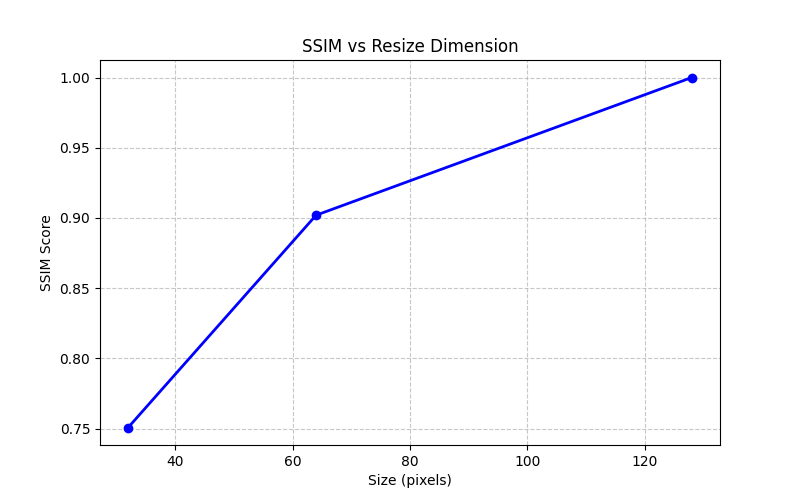
\includegraphics[width=0.65\textwidth]{graphics/ssim_curve.png}
    \caption{Đường cong SSIM theo kích thước resize; điểm tham chiếu là ảnh
        $128 \times 128$.}
    \label{fig:ssim_curve}
\end{figure}

Tại kích thước $32 \times 32$, SSIM đạt 0,7507 và PSNR đạt 26,09\,dB, phản
ánh mức độ mất mát thông tin cấu trúc đáng kể so với ảnh tham chiếu. Kích
thước $64 \times 64$ cải thiện đáng kể với SSIM = 0,9019 và PSNR = 30,47\,dB,
trong khi $128 \times 128$ được chọn làm kích thước làm việc thống nhất vì bảo
toàn toàn vẹn cấu trúc ảnh và phù hợp với yêu cầu đầu vào của các kiến trúc
học sâu được khảo sát. Phép co ảnh sử dụng nội suy \texttt{cv2.INTER\_AREA}
nhằm tối thiểu hóa hiện tượng răng cưa.

\paragraph{Chuẩn hóa không gian màu.}
Toàn bộ ảnh được chuyển về không gian màu \texttt{RGB} thông qua phép chuyển
đổi \texttt{BGR}$\rightarrow$\texttt{RGB}, đảm bảo tính đồng nhất về kênh màu
trên toàn tập dữ liệu. Nhóm đồng thời khảo sát hiệu quả biểu diễn đặc trưng
của bốn không gian màu thông qua phân tích thành phần chính PCA ($k = 50$) và
độ chính xác $k$-NN ($k = 5$) (Bảng~\ref{tab:color_space},
Hình~\ref{fig:color_space_pca}).

\begin{table}[H]
    \centering
    \caption{Phương sai giải thích tích lũy (PCA, $k=50$) và độ chính xác phân
        loại theo không gian màu ($k$-NN, $k=5$)}
    \label{tab:color_space}
    \begin{tabular}{lcc}
        \hline
        \textbf{Không gian màu} & \textbf{Phương sai giải thích tích lũy}
            & \textbf{Độ chính xác} \\
        \hline
        RGB       & 82,56\% & 45,19\% \\
        Grayscale & 85,21\% & 43,27\% \\
        HSV       & 73,67\% & 50,96\% \\
        LAB       & 82,69\% & 42,31\% \\
        \hline
    \end{tabular}
\end{table}

\begin{figure}[H]
    \centering
    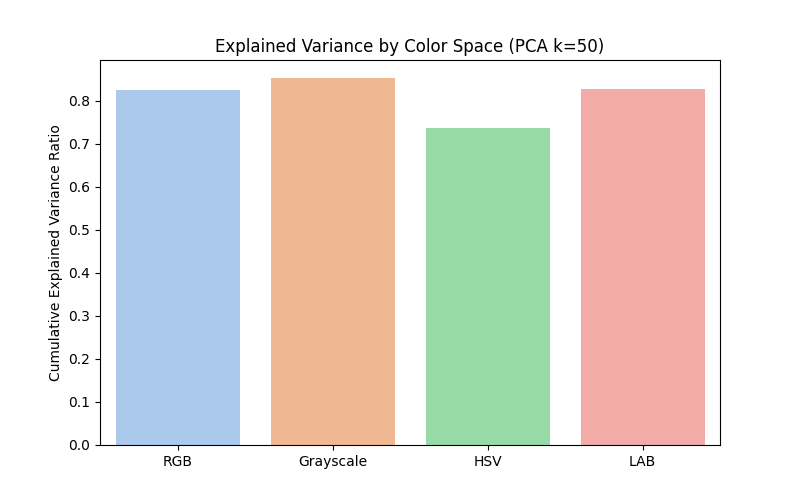
\includegraphics[width=0.7\textwidth]{graphics/color_space_pca.png}
    \caption{Phương sai giải thích tích lũy của PCA ($k=50$) theo từng không
        gian màu.}
    \label{fig:color_space_pca}
\end{figure}

Không gian \texttt{Grayscale} đạt phương sai giải thích tích lũy cao nhất
(85,21\%) với chỉ 50 thành phần, song lại cho độ chính xác phân loại thấp nhất
(43,27\%), phản ánh sự mất mát thông tin kênh màu có giá trị phân biệt lớp.
Không gian \texttt{HSV} đạt độ chính xác cao nhất (50,96\%) mặc dù phương sai
giải thích tích lũy thấp nhất (73,67\%), cho thấy không gian màu này tách biệt
tốt hơn theo thành phần sắc độ (Hue) đặc thù của từng nhãn. \texttt{RGB} được
chọn cho quy trình huấn luyện chính vì đây là không gian màu chuẩn đầu vào của
các kiến trúc học sâu được sử dụng và đảm bảo tính tái lập kết quả.

\subsubsection{Chuẩn hóa giá trị điểm ảnh}

Nhóm khảo sát bốn phương pháp chuẩn hóa nhằm đánh giá tác động đến khả năng
phân loại (Bảng~\ref{tab:normalization}).

\begin{table}[H]
    \centering
    \caption{Các phương pháp chuẩn hóa giá trị điểm ảnh được khảo sát}
    \label{tab:normalization}
    \begin{tabular}{llc}
        \hline
        \textbf{Phương pháp} & \textbf{Công thức} & \textbf{Miền giá trị} \\
        \hline
        Min-Max {[}0,\,1{]}       & $(x - x_{\min}) / (x_{\max} - x_{\min})$
            & $[0,\;1]$ \\
        Min-Max {[}-1,\,1{]}      & $2(x - x_{\min}) / (x_{\max} - x_{\min}) - 1$
            & $[-1,\;1]$ \\
        Chuẩn hóa $z$ toàn cục   & $(x - \mu_{\text{global}}) / \sigma_{\text{global}}$
            & $(-\infty,+\infty)$ \\
        Chuẩn hóa $z$ theo kênh  & $(x_c - \mu_c) / \sigma_c,\;\forall c \in \{R,G,B\}$
            & $(-\infty,+\infty)$ \\
        \hline
    \end{tabular}
\end{table}

Kiểm định Kolmogorov--Smirnov giữa phân phối gốc và phân phối sau chuẩn hóa
$z$ toàn cục cho $p \approx 0$ (dưới ngưỡng biểu diễn số thực của máy), xác
nhận sự khác biệt có ý nghĩa thống kê cao giữa hai phân phối. Tuy nhiên,
ablation study (Bảng~\ref{tab:norm_ablation}) cho thấy độ chính xác của bộ
phân lớp $k$-NN ($k = 5$) không thay đổi giữa các phương pháp, đồng nhất ở
mức 45,19\%. Kết quả này phản ánh giới hạn nội tại của đặc trưng thô khi chưa
qua chiết xuất sâu: phép chuẩn hóa thay đổi tỉ lệ nhưng không tạo ra sự tách
biệt tuyến tính mới trong không gian điểm ảnh phẳng.

\begin{table}[H]
    \centering
    \caption{Độ chính xác phân loại theo phương pháp chuẩn hóa
        (bộ phân lớp $k$-NN, $k=5$)}
    \label{tab:norm_ablation}
    \begin{tabular}{lc}
        \hline
        \textbf{Phương pháp} & \textbf{Độ chính xác} \\
        \hline
        Không chuẩn hóa          & 45,19\% \\
        Min-Max {[}0,\,1{]}      & 45,19\% \\
        Min-Max {[}-1,\,1{]}     & 45,19\% \\
        Chuẩn hóa $z$ toàn cục  & 45,19\% \\
        Chuẩn hóa $z$ theo kênh & 45,19\% \\
        \hline
    \end{tabular}
\end{table}

\subsubsection{Tăng cường dữ liệu}

Để nâng cao tính đa dạng của tập huấn luyện và giảm thiểu hiện tượng khớp quá
mức, nhóm áp dụng quy trình tăng cường dữ liệu bằng thư viện
\texttt{albumentations} với sáu phép biến đổi ngẫu nhiên
(Bảng~\ref{tab:augmentation}). Quy trình chỉ được áp dụng trên tập huấn luyện;
tập kiểm định và tập kiểm thử giữ nguyên dữ liệu gốc nhằm đảm bảo tính khách
quan trong đánh giá.

\begin{table}[H]
    \centering
    \caption{Quy trình tăng cường dữ liệu hình ảnh}
    \label{tab:augmentation}
    \begin{tabular}{p{4cm}p{3.5cm}p{7cm}}
        \hline
        \textbf{Phép biến đổi} & \textbf{Tham số} & \textbf{Lý giải} \\
        \hline
        Lật ngang ngẫu nhiên
            & $p = 0{,}5$
            & Vết hư hỏng trên bao bì có tính đối xứng không gian; phép
              lật không làm thay đổi nhãn phân loại. \\[4pt]
        Lật dọc ngẫu nhiên
            & $p = 0{,}5$
            & Bổ sung tính bất biến với hướng chụp theo trục dọc. \\[4pt]
        Xoay ngẫu nhiên
            & $\text{limit} = \pm 30^{\circ}$, $p = 0{,}5$
            & Mô phỏng độ lệch góc chụp thực tế; giá trị giới hạn đủ nhỏ
              để bảo toàn đặc trưng hình dạng bao bì. \\[4pt]
        Cắt và co giãn ngẫu nhiên
            & $\text{scale} \in [0{,}7;\,1{,}0]$, $p = 0{,}5$
            & Tạo tính bất biến với vị trí và tỉ lệ vật thể trong
              khung hình. \\[4pt]
        Nhiễu Gaussian ngẫu nhiên
            & $\sigma^2 \in [10;\,50]$, $p = 0{,}5$
            & Mô phỏng nhiễu cảm biến trong điều kiện ánh sáng yếu
              hoặc chất lượng thiết bị thu thấp. \\[4pt]
        Biến đổi độ sáng và độ tương phản
            & $\Delta b = 0{,}2$, $\Delta c = 0{,}2$, $p = 0{,}5$
            & Mô phỏng sự chênh lệch điều kiện chiếu sáng giữa các môi
              trường thu thập dữ liệu khác nhau. \\
        \hline
    \end{tabular}
\end{table}

Đánh giá tác động qua biểu đồ $t$-SNE (Hình~\ref{fig:augmentation_tsne}) và
bộ phân lớp $k$-NN ($k = 5$) cho thấy độ chính xác trên tập tăng cường giảm
từ 45,19\% xuống 40,38\%. Sự sụt giảm này phù hợp với kỳ vọng lý thuyết: tăng
cường dữ liệu làm tăng phương sai của không gian đặc trưng, khiến bộ phân lớp
tuyến tính đơn giản khó phân tách hơn, song lại có lợi cho các mô hình học sâu
thông qua việc tiếp xúc với nhiều biến thể hình ảnh hơn trong quá trình huấn
luyện.

\begin{figure}[H]
    \centering
    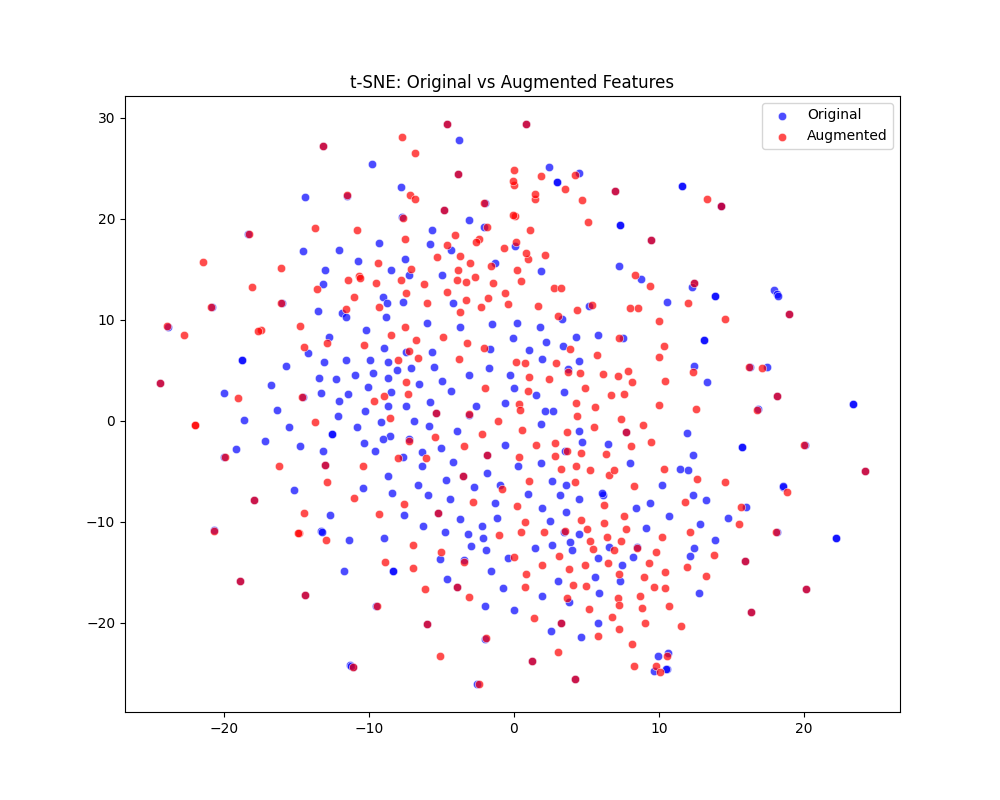
\includegraphics[width=0.7\textwidth]{graphics/augmentation_tsne.png}
    \caption{Biểu đồ $t$-SNE so sánh phân bố đặc trưng của tập ảnh gốc và tập
        ảnh sau tăng cường.}
    \label{fig:augmentation_tsne}
\end{figure}
\subsection{Kiểm tra sự nhất quán của dữ liệu}

Sau khi tiền xử lý, nhóm thực hiện các kiểm tra nhất quán (consistency checks):

\begin{itemize}[labelsep=10pt, leftmargin=2cm]
    \item Kiểm tra chéo trường dữ liệu: đảm bảo \texttt{rating} và nhãn cảm xúc nhất quán (ví dụ: rating 1 không thể gán nhãn ``tích cực'').
    \item Căn chỉnh ảnh và văn bản: kiểm tra mỗi \texttt{review\_id} trong CSV đều có thư mục ảnh tương ứng (nếu trường \texttt{images} không rỗng).
    \item Kiểm tra schema: dùng Pydantic model để validate từng bản ghi JSON đầu ra của scraper.
\end{itemize}

\clearpage
